\documentclass[]{standalone}

%\usepackage{mathptmx}
%\renewcommand{\familydefault}{\rmdefault}
%\usepackage[T1]{fontenc}
%\usepackage[latin9]{inputenc}
\usepackage{siunitx}
\usepackage{array}
\usepackage{amsmath}
\usepackage{ifthen}
\usepackage{pgfplots}
\pgfplotsset{compat=1.14}
\usepackage{titling, graphicx}
\usepackage{tikz}
\usepackage{upgreek}
\usepackage{amsmath,amsthm}
\usepackage{strtikz}
\usepackage{circledsteps}
\usetikzlibrary{shapes,arrows.meta,intersections,graphs,graphs.standard}
\usetikzlibrary{bending, math,fit}
\usetikzlibrary{calc,intersections,through,backgrounds}
\usetikzlibrary{decorations.markings,decorations.pathmorphing, decorations.pathreplacing}
\usetikzlibrary{patterns}



\begin{document}
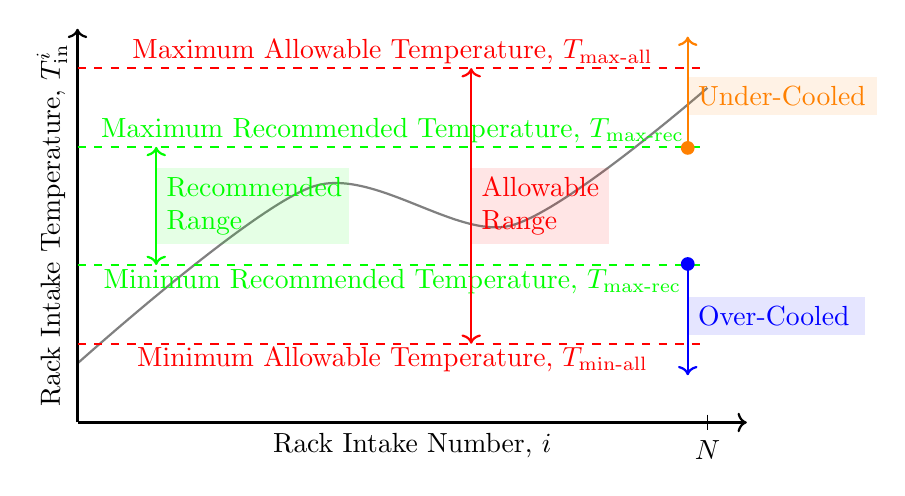
\begin{tikzpicture}[line join=round]

\draw[thick, gray] plot [smooth] coordinates {(0,0.75)  (3,3) (5.5,2.5) (8,4.25)};

\draw[->, thick] (0,0)  -- node[below] {Rack Intake Number, $i$}(8.5,0);
\draw[->, thick] (0,0)  -- node[above, rotate=90] {Rack Intake Temperature, $T_\text{in}^i$}(0,5);

\draw[] (8, 0.1) -- node[at end, anchor=north] {$N$} +(0,-0.2);

\draw[dashed, red, thick] (0, 4.5) -- node[above, inner sep=1pt]{Maximum Allowable Temperature, $T_{\text{max-all}}$} +(8,0);
\draw[dashed, red, thick] (0, 1.0) -- node[below, inner sep=1pt]{Minimum Allowable Temperature, $T_{\text{min-all}}$} +(8,0);

\draw[dashed, green, thick] (0, 3.5) -- node[above, inner sep=1pt]{Maximum Recommended Temperature, $T_{\text{max-rec}}$} +(8,0);
\draw[dashed, green, thick] (0, 2.0) -- node[below, inner sep=1pt]{Minimum Recommended Temperature, $T_{\text{max-rec}}$} +(8,0);

\draw[<->, green, thick] (1,2) -- node[anchor=west, text width=2.2cm, fill=green, opacity=0.1, text opacity=1]
{Recommended\\Range} +(0,1.5);

\draw[<->, red, thick] (5,1) -- node[anchor=west, text width=1.5cm, fill=red, opacity=0.1, text opacity=1]
{Allowable\\Range} +(0,3.5);

\draw[{Circle[]}->, thick, blue] (7.75, 2.1) -- node[anchor=west, text width=2cm, fill=blue, opacity=0.1, text opacity=1]
{Over-Cooled} +(0,-1.5);

\draw[{Circle[]}->, thick, orange] (7.75, 3.4) -- node[anchor=west, text width=2.15cm, fill=orange, opacity=0.1, text opacity=1]
{Under-Cooled} +(0, 1.5);

\end{tikzpicture}
\end{document}
